\chapter{Arrays}

\section{Qué son y cómo crear \emph{arrays}}
Las variables pueden ser valores escalares, como en el ejemplo de la sección anterior, o también series organizadas de valores (\emph{arrays}), que pueden tener varias dimensiones (matrices o hipermatrices, que formalmente reciben el nombre de \emph{multi-dimensional arrays}). Su definición y uso no es uno de los aspectos más sencillos del lenguaje, y de hecho acarrea bastantes complicaciones, pero conviene introducirlos en este punto ya que hay muchos otros conceptos que se entienden mejor habiendo conocido lo que son y cómo son los \emph{arrays}, o incluso no se pueden entender de otra manera. Además, los \emph{arrays} son un elemento fundamental para la mayoría de cálculos numéricos, por lo que tiene doble sentido hablar de ellos desde un principio.

Un \emph{array} se define entre corchetes, con cada valor individual separado por comas:

\begin{jlconcode}
julia> primos = [1,2,3,5,7,11]
6-element Array{Int64,1}:
 1
 2
 3
 5
 7
 11
\end{jlconcode}

Como se comprueba en este ejemplo, los \emph{arrays} unidimensionales son equivalentes a ``vectores columna''. Por lo tanto, en la práctica la coma puede sustituirse por el punto y coma (\code{;}), que se utiliza como forma abreviada de la función \code{vcat} (``concatenación vertical''). Pero no es legal combinar la coma y el punto y coma de forma indiscriminada:

\begin{jlconcode}
julia> # Comparar definición con puntos y comas
julia> primos == [1;2;3;5;7;11]
true

julia> # Sintaxis errónea
julia> [1,2;3]
ERROR: syntax: unexpected semicolon in array expression
\end{jlconcode}

En matrices de más de una dimensión, las columnas se concatenan horizontalmente mediante la función \code{hcat}, o más compactamente mediante espacios:

\begin{jlconcode}
julia> # Equivale a mat = hcat([1,2,3], [10,20,30], [0.1,0.2,0.3])
julia> mat = [[1,2,3] [10,20,30] [0.1,0.2,0.3]]
3x3 Array{Float64,2}:
 1.0 10.0 0.1
 2.0 20.0 0.2
 3.0 30.0 0.3
\end{jlconcode}

Por otro lado, para construir matrices siguiendo la habitual definición ``línea a línea'', los valores de cada línea se separan con espacios, y las líneas se separan entre sí mediante el punto y coma (también se puede usar la función \code{hvcat}, especificando cuántas columnas tiene cada línea):

\begin{jlconcode}
julia> # Equivale a mat = hvcat(3, 1, 10, 0.1, 2, 20, 0.2, 3, 30, 0.3)
julia> mat = [1 10 0.1; 2 20 0.2; 3 30 0.3]
3x3 Array{Float64,2}:
 1.0 10.0 0.1
 2.0 20.0 0.2
 3.0 30.0 0.3
\end{jlconcode}

Otras operaciones útiles para la construcción de matrices son la transposición (con la función \code{transpose} o el operador apóstrofe \textinline{'}), la función \code{cat}, que se utiliza de forma general para concatenar series o matrices en cualquier dimensión, más allá de las dos primeras (filas o columnas), y la función \code{reshape}, para reorganizar las dimensiones de un \emph{array}.


\section{Indexación y manipulación. Variables de tipo ``rango''}

Para leer o modificar un valor de un \emph{array}, se indexa la posición seleccionar entre corchetes(\code{[]}), siguiendo el orden fila-columna-etc. (la primera posición se indica con el número 1). Si solo se utiliza un índice de posición, hay que tener en cuenta que los valores están internamente ordenados por columnas:

\begin{jlconcode}
julia> # Cuarto número primo:
julia> primos[4]
5

julia> # Primera fila, segunda columna de mat:
julia> mat[1, 2]
10

julia> # O lo que es lo mismo, primer valor tras la primera columna:
julia> mat[3 + 1]
10
\end{jlconcode}

Se pueden utilizar vectores de índices, para seleccionar varios valores o combinaciones de filas y columnas en la misma operación. Por ejemplo, para intercambiar la segunda y tercera filas de \code{mat} (completas, es decir los valores de las tres columnas para esas dos filas):

\begin{jlconcode}
julia> # Véase que los índices de las filas se invierten al reasignarlos:
julia> mat[[2,3],[1,2,3]] = mat[[3,2],[1,2,3]];
julia> mat
3x3 Array{Float64,2}:
 1 10 0.1
 3 30 0.3
 2 20 0.2
\end{jlconcode}

Estos conjuntos de índices se pueden escribir de forma más cómoda a través de ``rangos'' (\emph{ranges}), un tipo especial de variable que representa una serie aritmética acotada. Los rangos se definen a través de tres valores: el primero y último de la serie (\code{a} y \code{b}, respectivamente), más el ``paso'' o diferencia entre dos números consecutivos (\code{s}), con la sintaxis \code{a:s:b}. Por ejemplo, la serie de números impares entre 1 y 10:

\begin{jlconcode}
julia> impares = 1:2:10
1:2:9
\end{jlconcode}
En este ejemplo el valor final asignado (10) no es compatible con la definición del valor inicial y el paso, por lo tanto se sustituye automáticamente por 9, el valor compatible más cercano (\emph{dentro} del rango entre los valores inicial y final asignados). El conjunto de valores representados se entiende más fácilmente si el resultado se convierte a un vector, usando la operación \code{collect}:

\begin{jlconcode}
julia> collect(impares)
5-element Array{Int64,1}:
 1
 3
 5
 7
 9
\end{jlconcode}

Los números de un rango no han de ser necesariamente enteros ni positivos, aunque es lo lógico cuando se quiere definir un conjunto de índices. Por otro lado, el paso \code{s} es un valor opcional, que por defecto se asume igual a 1. Para construir una serie ordenada de mayor a menor, además de definir los valores inicial y final en el orden adecuado, se ha de definir un paso negativo. Olvidar este detalle hace que la serie creada sea vacía. Por ejemplo, para una ``cuenta atrás'' de 5 a 1 (convertida a vector para más claridad):

\begin{jlconcode}
julia> collect(5:-1:1) # Correcto
5-element Array{Int64,1}:
 5
 4
 3
 2
 1 

julia> collect(5:1) # Serie vacía
0-element Array{Int64,1}:
\end{jlconcode}

Algunos trucos útiles con rangos cuando se usan como índices son: la palabra clave \code{end} hace referencia a la última posición/fila/columna indexable en el \emph{array} manipulado; y los dos puntos aislados (\code{:}) hacen referencia a ``todas'' las posiciones, filas o columnas.

\begin{jlconcode}
julia> # Serie de números primos al revés:
julia> primos[end:-1:1]
6-element Array{Int64,1}:
 11
 7
 5
 3
 2
 1

julia> # Intercambiar las filas primera y segunda (antes tercera) de mat
julia> mat[1:2,:] = mat[[2,1],:];
julia> mat
3x3 Array{Float64,2}:
 3 30 0.3
 1 10 0.1
 2 20 0.2
\end{jlconcode}

\section{Dificultades de los \emph{arrays}. 1: ``mutabilidad''}

Es importante tener en cuenta que los \emph{arrays} en Julia no son solo agrupaciones de valores para manejarlos de forma conjunta. Son un tipo de variable diferente a los valores escalares, que muestra un comportamiento distinto. Para empezar, es lo que se llama un objeto ``mutable''; por ejemplo se pueden cambiar uno o más valores del \emph{array} manteniendo el resto sin alterar. Esto hay que tenerlo en cuenta cuando se ``copian'' variables, porque puede llevar a resultados inesperados. Por ejemplo:

\begin{jlconcode}
julia> sa = [1, 2, 3];
julia> # Creamos otro array sb "igual a sa"
julia> sb = sa;
julia> # Ahora modificamos sa...
julia> sa[1] = 0;
julia> # Volvemos a cambiar su contenido, multiplicándolo por 10
julia> sa = sa*10;
julia> # Esto es lo que podía esperarse
julia> sa
3-element Array{Int64,1}:
  0
 20
 30

julia> # ¿Pero por qué sb no coincide con el contenido inicial de sa?
julia> sb
3-element Array{Int64,1}:
 0
 2
 3
\end{jlconcode}

Una forma de entender lo que pasa en este ejemplo es considerar que las variables \code{sa}, \code{sb} no son lo mismo que los objetos contenidos en ellas (en este caso los \emph{arrays}), sino meras referencias, una especie de ``etiquetas'' que pueden asignarse de forma independiente, e incluso redundante a los diversos objetos que hay en el espacio de trabajo. La figura \ref{fig:arrays-asignacion-modificacion} muestra gráficamente lo que ocurre en cada una de las operaciones.

\begin{figure}
\centering
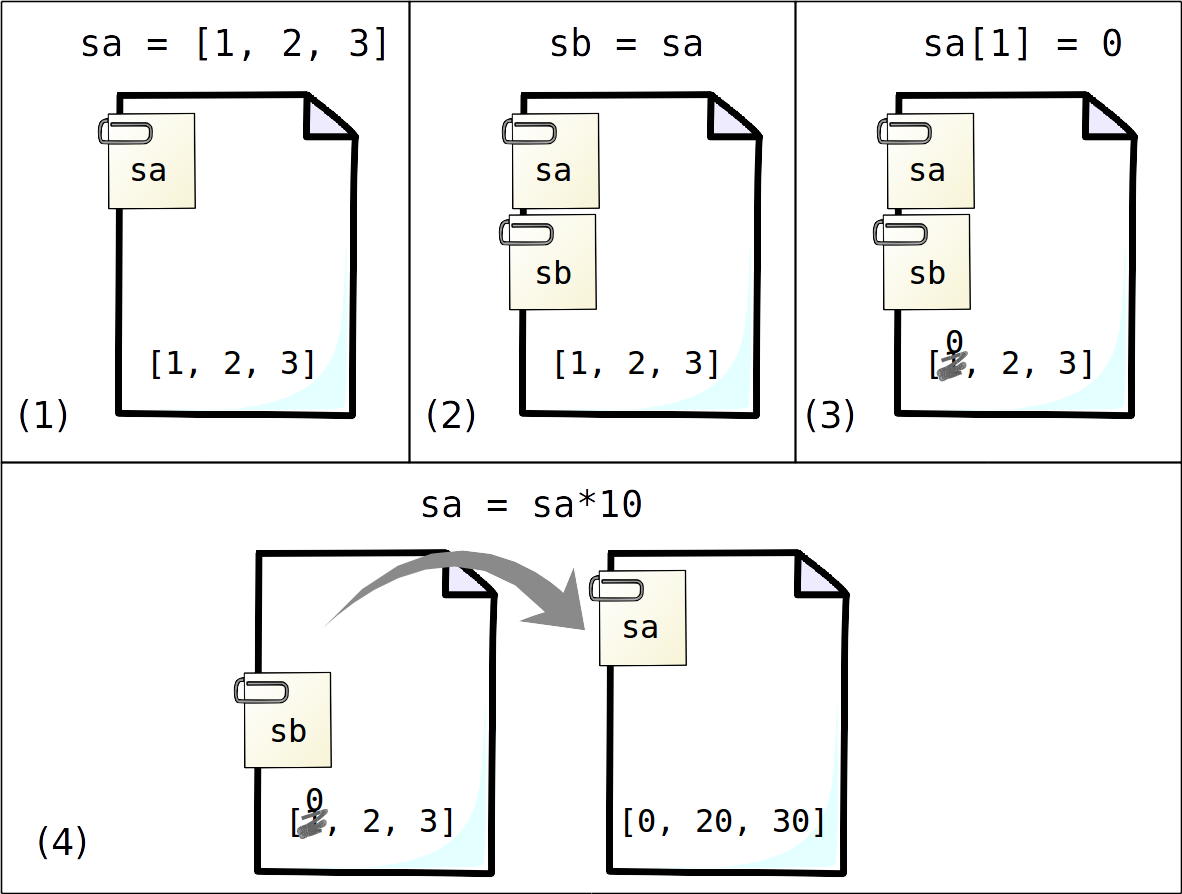
\includegraphics[scale=1.5]{arrays-asignacion-modificacion}
\caption{Representación gráfica de las operaciones de Julia para: (1) asignar un vector a la variable \code{sa}; (2) asignar el contenido de \code{sa} a \code{sb}; (3) modificar el contenido de \code{sa}; (3) asignar un nuevo valor a \code{sa}.}
\label{fig:arrays-asignacion-modificacion}
\end{figure}

Como los \emph{arrays} son elementos mutables, al hacer que \code{sb} se identifique con \code{sa}, los cambios realizados a una de las variables afecta también a la otra ---a no ser que una de las variables se reasigne, como ocurre en el cuarto paso.

Este comportamiento se puede evitar definiendo los \emph{arrays} explícitamente como ``copias'' de otros. La forma más concisa es haciendo referencia a todos los valores individuales (con \code{[:]}).

\begin{jlconcode}
julia> # sa se redefine como un array que contiene "todos los valores de sb"
julia> sa = sb[:]
3-element Array{Int64,1}:
 0
 2
 3

julia> # Si redefinimos el primer elemento de sa, el cambio ya no se aplica a sb
julia> sa[1] = 1;
julia> sa
3-element Array{Int64,1}:
 1
 2
 3

julia> sb
3-element Array{Int64,1}:
 0
 2
 3
\end{jlconcode}


\section{Dificultades de los \emph{arrays}. 2: Restricciones de tipo y tamaño.}

Además, el tipo de datos y las dimensiones de un \emph{array} son fijos (aunque sí se le puede reasignar un conjunto de datos nuevo, con otro tipo de datos u otro tamaño). La restricción sobre los tipos de datos puede causar ciertos problemas, ya que los números pueden codificarse de varias maneras, y puede crearse de forma accidental un \emph{array} con un tipo distinto del que se realmente se pretende utilizar. Por eso, al presentar un \emph{array} en pantalla siempre se muestra el tipo de datos y las dimensiones asociadas; en los ejemplos anteriores se han usado los tipos \code{Int64} (enteros de 32 bits) y \code{Float64} (números decimales de doble precisión --- 64 bits ---). Estos son los tipos por defecto creados en un sistema operativo de 32 bits (en uno de 64 bits los enteros serían \code{Int64}, aunque los decimales serían iguales), según los valores asignados en la creación. También se puede consultar el tipo de una variable (\emph{array} u otro tipo) con la función \code{typeof}.

El problema mencionado se puede ejemplificar con los \emph{arrays} \code{sa} y \code{sb}, que se habían definido a partir de secuencias de números enteros, y por lo tanto son \emph{arrays} del tipo \code{Int64}. Esto significa que asignar un valor decimal a un elemento sería ilegal:

\begin{jlconcode}
julia> sa[1] = 0.5
ERROR: InexactError()
 in setindex! at array.jl:313
\end{jlconcode}

Si se hubiera querido crear una secuencia de 1 a 3 con números decimales, habría varias alternativas:

\begin{jlconcode}
julia> # 1. Declarar el tipo de datos del vector en su creación
julia> sf = Float64[1,2,3];
julia> typeof(sf)
Array{Float64,1}

julia> # 2. Crear primero el vector declarando el tipo de datos y el tamaño
julia> sf = Array(Float64, 3);
julia> sf[:] = [1,2,3];
julia> typeof(sf)
Array{Float64,1}

julia> # 3. Convertir la secuencia de enteros explícitamente a tipo float
julia> sf = float([1,2,3]);
julia> typeof(sf)
Array{Float64,1}

julia> # 4. Introducir números explícitamente decimales al definir la secuencia
julia> # (vale con que un solo valor sea decimal)
julia> sf = [1.0, 2, 3];
julia> typeof(sf)
Array{Float64,1}
\end{jlconcode}

El truco de la última opción consiste en aprovechar la ``promoción'' automática que realiza Julia al operar con una combinación de números enteros y decimales, por virtud de la cual los enteros se tratan como si fueran decimales. (Véase la sección XXXXX para más detalles sobre los tipos.)

Julia admite muchos otros tipos de datos; los básicos son enteros con o sin signo y números decimales de distintas precisiones, pero hay muchas más abstracciones, incluyendo números racionales y complejos. Y hay también un ``supertipo'' \code{Any}, que incluye todos los tipos de objetos que pueden existir en Julia. Las variables escalares también se clasifican según dichos tipos, aunque en su caso la asignación no muestra estos problemas. Puede consultarse el manual de Julia para un catálogo completo de los tipos numéricos básicos y las reglas de promoción entre ellos.

Vista ya la cuestión de las restricciones de tipo, el otro error típico a la hora de manipular \emph{arrays} consiste en intentar la lectura o modificación de un valor más allá de su tamaño predefinido, aunque el \emph{array} siempre se puede cambiar por otro nuevo de mayor tamaño:

\begin{jlconcode}
julia> # Así no se puede añadir un cuarto valor a sa:
julia> sa[4] = 4
ERROR: BoundsError()

julia> # Se puede concatenar sa con el cuarto valor, y reasignar el resultado:
julia> sa = [sa, 4]
4-element Array{Int64,1}:
 1 
 2 
 3 
 4
\end{jlconcode}

Otra forma de ampliar \emph{arrays} es usar funciones como \code{push!}, \code{append!}, \code{unshift!}, \code{prepend!}, \code{insert!}, \code{resize!}, etc. (el signo \code{!} en el nombre es una convención para indicar que la función modifica el argumento). También hay funciones complementarias para eliminar elementos del \emph{array}, como \code{pop!}, \code{shift!} o \code{splice!}, que además devuelven el valor del elemento extraído. Es típico crear \emph{arrays} que se van ampliando progresivamente en procesos iterativos, pero en la medida de lo posible es recomendable definirlos en un primer momento con el tamaño necesario para contener todos los elementos que requiera, sobredimensionándolo si hace falta y ``recortándolos'' después si se quiere. Esto evita la creación de una nueva variable en cada iteración, que puede consumir más tiempo de procesado que las demás operaciones, y reduce potencialmente el coste computacional en varios órdenes de magnitud.

\section{Operaciones matriciales}

Un caso especial de los \emph{arrays} es de las matrices bidimensionales, que son un elemento fundamental del álgebra lineal. (En el resto de esta sección se hablará simplemente de ``matrices'' sobreentendiéndose el calificativo de ``bidimensional''). La relevancia de las matrices implica que hay una cantidad muy importante de operaciones matemáticas dirigidas a este tipo de variables, y que no son válidas para \emph{arrays} de más dimensiones.

Por ejemplo, las operaciones de multiplicación y división en ambos sentidos (\code{*}, \code{/}, \textinline{\}), así como la potenciación por un escalar (\code{^}) se interpretan como operaciones específicas para matrices. También pueden aplicarse a escalares o vectores unidimensionales, aunque esto se debe a que pueden considerarse matrices de tamaño $1\times{}1$ o de una sola columna, respectivamente.

Sin embargo, estas operaciones también podrían querer aplicarse a cada elemento individual del \emph{array} (o \emph{arrays}) de entrada. Por ese motivo, existe una versión ``elemento-a-elemento'' de esos operadores, que se distinguen por un punto precedente (\code{.*}, \code{./}, \textinline{.\}).

También existe esta versión para operadores de comparación (\code{.==}, \code{.!=}, etc.), así como para  la suma y la resta (\code{.+}, \code{.-}, respectivamente), aunque la definición matricial y elemento a elemento de estas dos últimas no tiene distinción. De hecho, las sumas y restas ``con punto'' y ``sin punto'' sirven igualmente para todo tipo de \emph{arrays} (si las dimensiones de los operandos son iguales). La principal diferencia consiste en que las versiones con punto hacen una expansión automática de los operandos (\emph{broadcasting}) si algunas dimensiones son unitarias. Por ejemplo:

\begin{jlconcode}
julia> # Filas con unidades distintas, columnas con decimales distintos
julia> # Solo se suma un vector columna más un vector fila
julia> [1,2,3] .+ [0.1 0.2 0.3]
3x3 Array{Float64,2}:
 1.1 1.2 1.3
 2.1 2.2 2.3
 3.1 3.2 3.3
\end{jlconcode}

Este truco no tiene lugar en la suma ``sin punto'', que por otro lado es más rápida. Por lo tanto, si se busca seguridad ante errores de programación (evitar expansiones si por accidente se suman \emph{arrays} de dimensiones incoherentes) y eficiencia en el procesado, es preferible usar la versión sin punto. La expansión automática siempre puede forzarse de forma eficiente con la función \code{broadcast}.

Para las funciones ``con nombre'' que tienen una definición matricial específica, como la exponencial, el criterio es el contrario: la función con el nombre ``normal'' (\code{exp}) hace la operación elemento a elemento cuando se aplica a cualquier tipo de \emph{array}; y se utiliza un nombre especial para la operación matricial (\code{expm}).

Muchas otras funciones (p.ej. las funciones trigonométricas) solo tienen sentido en \emph{arrays} si se hacen elemento a elemento, y por lo tanto son válidas tal cual con el mismo nombre para \emph{arrays} y para escalares.


